\documentclass[a4paper, 12pt]{article}
\usepackage[utf8]{inputenc}

\usepackage[a4paper,top=1.3cm,bottom=2cm,left=1.5cm,right=1.5cm,marginparwidth=0.75cm]{geometry}
\usepackage{cmap}				
\usepackage{mathtext} 				
\usepackage[T2A]{fontenc}			
\usepackage[utf8]{inputenc}			
\usepackage[english,russian]{babel}	
\usepackage{multirow}
\usepackage{mathtools}
\mathtoolsset{showonlyrefs=true}

\usepackage{graphicx}
\usepackage{wrapfig}
\usepackage{tabularx}
\usepackage{caption}

\title{2.1.3-theory}
\author{Влад Черниенко}
\date{March 2022}


\begin{document}

    \begin{titlepage}
    
        \begin{center}
            {\large МОСКОВСКИЙ ФИЗИКО-ТЕХНИЧЕСКИЙ ИНСТИТУТ (НАЦИОНАЛЬНЫЙ ИССЛЕДОВАТЕЛЬСКИЙ УНИВЕРСИТЕТ)}
        \end{center}
        \begin{center}
            {\large Фихтех-школа радиотехники и компьютерных технологий}
        \end{center}
        
        \vspace{4.5cm}
        
        {\huge
            \begin{center}
                {\bf Лабораторная работа 2.1.6} \\
                Эффект Джоуля-Томсона
            \end{center}
        }
        
        \vspace{12cm}
        
        \begin{flushright}
            {\LARGE Автор: \\ Черниенко Владислав Антонович \\ \vspace{0.2cm} Группа Б01-110}
        \end{flushright}
        
    \end{titlepage}
    
    
    \noindent {\bf Цель работы:} 1) определение изменения температуры углекислого газа при протекании через малопроницаемую перегородку при разных начальных значениях давления и температуры; 2) вычисление по результатам опытов коэффициентов Ван-дер-Ваальса «$a$» и «$b$».\\
    
    \noindent {\bf В работе используются:} трубка с пористой перегородкой; труба Дьюара; термостат; термометры; дифференциальная термопара; микровольтметр; балластный баллон; манометр.\\
    
    \begin{flushleft}
        {\Large {\bf Теоретические сведения}}
    \end{flushleft}
    
    Эффектом Джоуля–Томсона называется изменение температуры газа, медленно протекающего из области высокого в область низкого давления в условиях хорошей тепловой изоляции. В разреженных газах, которые приближаются по своим свойствам к идеальному газу, при таком течении температура газа не меняется. Эффект Джоуля–Томсона демонстрирует отличие исследуемого газа от идеального.
    
    В работе исследуется изменение температуры углекислого газа при медленном его течении по трубке с пористой перегородкой (рис. \ref{pic1}). Трубка 1 хорошо теплоизолирована. Газ из области повышенного давления $P_1$ проходит через множество узких и длинных каналов пористой перегородки 2 в область с атмосферным давлением $P_2$. Перепад давления $\Delta P = P_1 - P_2$ из-за большого сопротивления каналов может быть заметным даже при малой скорости течения газа в трубке. Величина эффекта Джоуля–Томсона определяется по разности температуры газа до и после перегородки.
    
    Рассмотрим стационарный поток газа между произвольными сечениями $I$ и $II$ трубки (до перегородки и после нее). Пусть, для определенности, через трубку прошел 1 моль углекислого газа; $\mu$ — его молярная масса. Молярные объемы газа, его давления и отнесенные к молю внутренние энергии газа в сечениях $I$ и $II$ обозначим соответственно $V_1$, $P_1$, $U_1$ и $V_2$, $P_2$, $U_2$. Для того чтобы ввести в трубку объем $V_1$, над газом нужно совершить работу $A_1 = P_1 V_1$. Проходя через сечение $II$, газ сам совершает работу $A_2 = P_2 V_2$. Так как через боковые стенки не происходит ни обмена теплом, ни передачи механической энергии, то
    \begin{equation}
        A_1 - A_2 = \left( U_2 + \frac{\mu v_2^2}{2} \right) - \left( U_1 + \frac{\mu v_1^2}{2} \right).
        \label{eq1}
    \end{equation}
    В уравнении \eqref{eq1} учтено изменение как внутренней (первые члены в скобках), так и кинетической (вторые члены в скобках) энергии газа. Подставляя в \eqref{eq1} написанные выражения для $A_1$ и $A_2$ и перегруппировывая члены, найдем
    \begin{equation}
        H_1 - H_2 = (U_1 + P_1 V_1) - (U_2 + P_2 V_2) = \frac{1}{2} \mu (v_2^2 - v_1^2).
        \label{eq2}
    \end{equation}
    
    Сделаем замечание, связанное с правой частью \eqref{eq2}. Процесс Джоуля–Томсона в чистом виде осуществляется лишь в том случае, если правой частью можно пренебречь, т. е. если макроскопическая скорость газа с обеих сторон трубки достаточно мала. У нас сейчас нет критерия, который позволил бы установить, когда это можно сделать. Поэтому мы отложим на некоторое время обсуждение вопроса о правой части \eqref{eq2}, а пока будем считать, что энтальпия газа не меняется.
    
    Используем выражение:
    \begin{equation}
        \mu_{д-т} = \frac{\Delta T}{\Delta P} \approx \frac{(2a / RT) - b}{C_p}.
        \label{eq3}
    \end{equation}
    Из формулы \eqref{eq3} видно, что эффект Джоуля–Томсона для не очень плотного газа зависит от соотношения величин $a$ и $b$, которые оказывают противоположное влияние на знак эффекта. Если силы взаимодействия между молекулами велики, так что превалирует «поправка на давление», то основную роль играет член, содержащий $a$, и
    \begin{equation}
        \frac{\Delta T}{\Delta P} > 0,
    \end{equation}
    т. е. газ при расширении охлаждается ($\Delta T < 0$, так как всегда $\Delta P < 0$). В обратном случае (малые $a$)
    \begin{equation}
        \frac{\Delta T}{\Delta P} < 0,
    \end{equation}
    т. е. газ нагревается ($\Delta T > 0$, так как по-прежнему $\Delta P < 0$).
    
    При температуре $T_i$ коэффициент $\mu_{д-т}$ обращается в нуль. Использую связь между коэффициентами $a$ и $b$ и критической температурой, по формуле
    \begin{equation}
        T_i = \frac{2a}{R b},
    \end{equation}
    найдём
    \begin{equation}
        T_{инв} = \frac{27}{4} T_{кр}.
        \label{eq4}
    \end{equation}
    При температуре $T_{инв}$ эффект Джоуля–Томсона меняет знак: ниже температуры инверсии эффект положителен ($\mu_{д-т} > 0$, газ охлаждается), выше $T_{инв}$ эффект отрицателен ($\mu_{д-т} < 0$, газ нагревается).
    
    Вернемся к влиянию правой части уравнения \eqref{eq2} на изменение температуры расширяющегося газа. Для этого сравним изменение температуры, происходящее вследствие эффекта Джоуля–Томсона, с изменением температуры, возникающим из-за изменения кинетической энергии газа. Увеличение кинетической энергии газа вызывает заметное и приблизительно одинаковое понижение его температуры как у реальных, так и у идеальных газов. Поэтому при оценках нет смысла пользоваться сложными формулами для газа Ван-дер-Ваальса.
    
    Заменяя в формуле \eqref{eq2} $U$ через $C_V T$ и $PV$ через $RT$, найдём
    \begin{equation}
        (R + C_V)(T_1 - T_2) = \mu (v_2^2 - v_1^2) / 2,
    \end{equation}
    или
    \begin{equation}
        \Delta T = \frac{\mu}{2 C_p} (v_2^2 - v_1^2).
    \end{equation}
    В условиях нашего опыта расход газа $Q$ на выходе из пористой перегородки не превышает 10 см$^3$/c, а диаметр трубки равен 3 мм. Поэтому
    \begin{equation}
        v_2 \leq \frac{4Q}{\pi d^2} = \frac{4 \cdot 10 \text{ см}^3\text{/с}}{3,14 \cdot (0,3)^2 \text{ см}^2} \approx 140 \text{ см/с}.
    \end{equation}
    Скорость $v_1$ газа у входа в пробку относится к скорости $v_2$ у выхода из нее как давление $P_2$ относится к $P_1$. В нашей установке $P_1 = 4$ атм, a $P_2 = 1$ атм, поэтому
    \begin{equation}
        v_1 = \frac{P_2}{P_1} v_2 = \frac{1 \text{ атм}}{4 \text{ атм}} \cdot 140 \text{ см/с} = 35 \text{ см/с}.
    \end{equation}
    Для углекислого газа $\mu = 44 \text{ г/моль}$, $C_p = 40 \text{ Дж/(моль} \cdot \text{К)}$; имеем
    \begin{equation}
        \Delta T = \frac{\mu}{2 C_p} (v_2^2 - v_1^2) = \frac{44 \cdot 10^{-3}}{2 \cdot 40} (1,4^2 - 0,28^2) = 7 \cdot 10^{-4} \text{ К}.
    \end{equation}
    Это изменение температуры ничтожно мало по сравнению с измеряемым эффектом (несколько градусов).
    
    В данной лабораторной работе исследуется коэффициент дифференциального эффекта Джоуля–Томсона для углекислого газа. По экспериментальным результатам оценивается коэффициент теплового расширения, постоянные в уравнении Ван-дер-Ваальса и температура инверсии углекислого газа. Начальная температура газа $T_1$ задается термостатом. Измерения будут проводиться при 6-7 значениях температуры.
    
    \newpage
    
    \begin{flushleft}
        {\Large {\bf Экспериментальная установка}}
    \end{flushleft}
    
    \begin{figure}[ht]
        \centering
        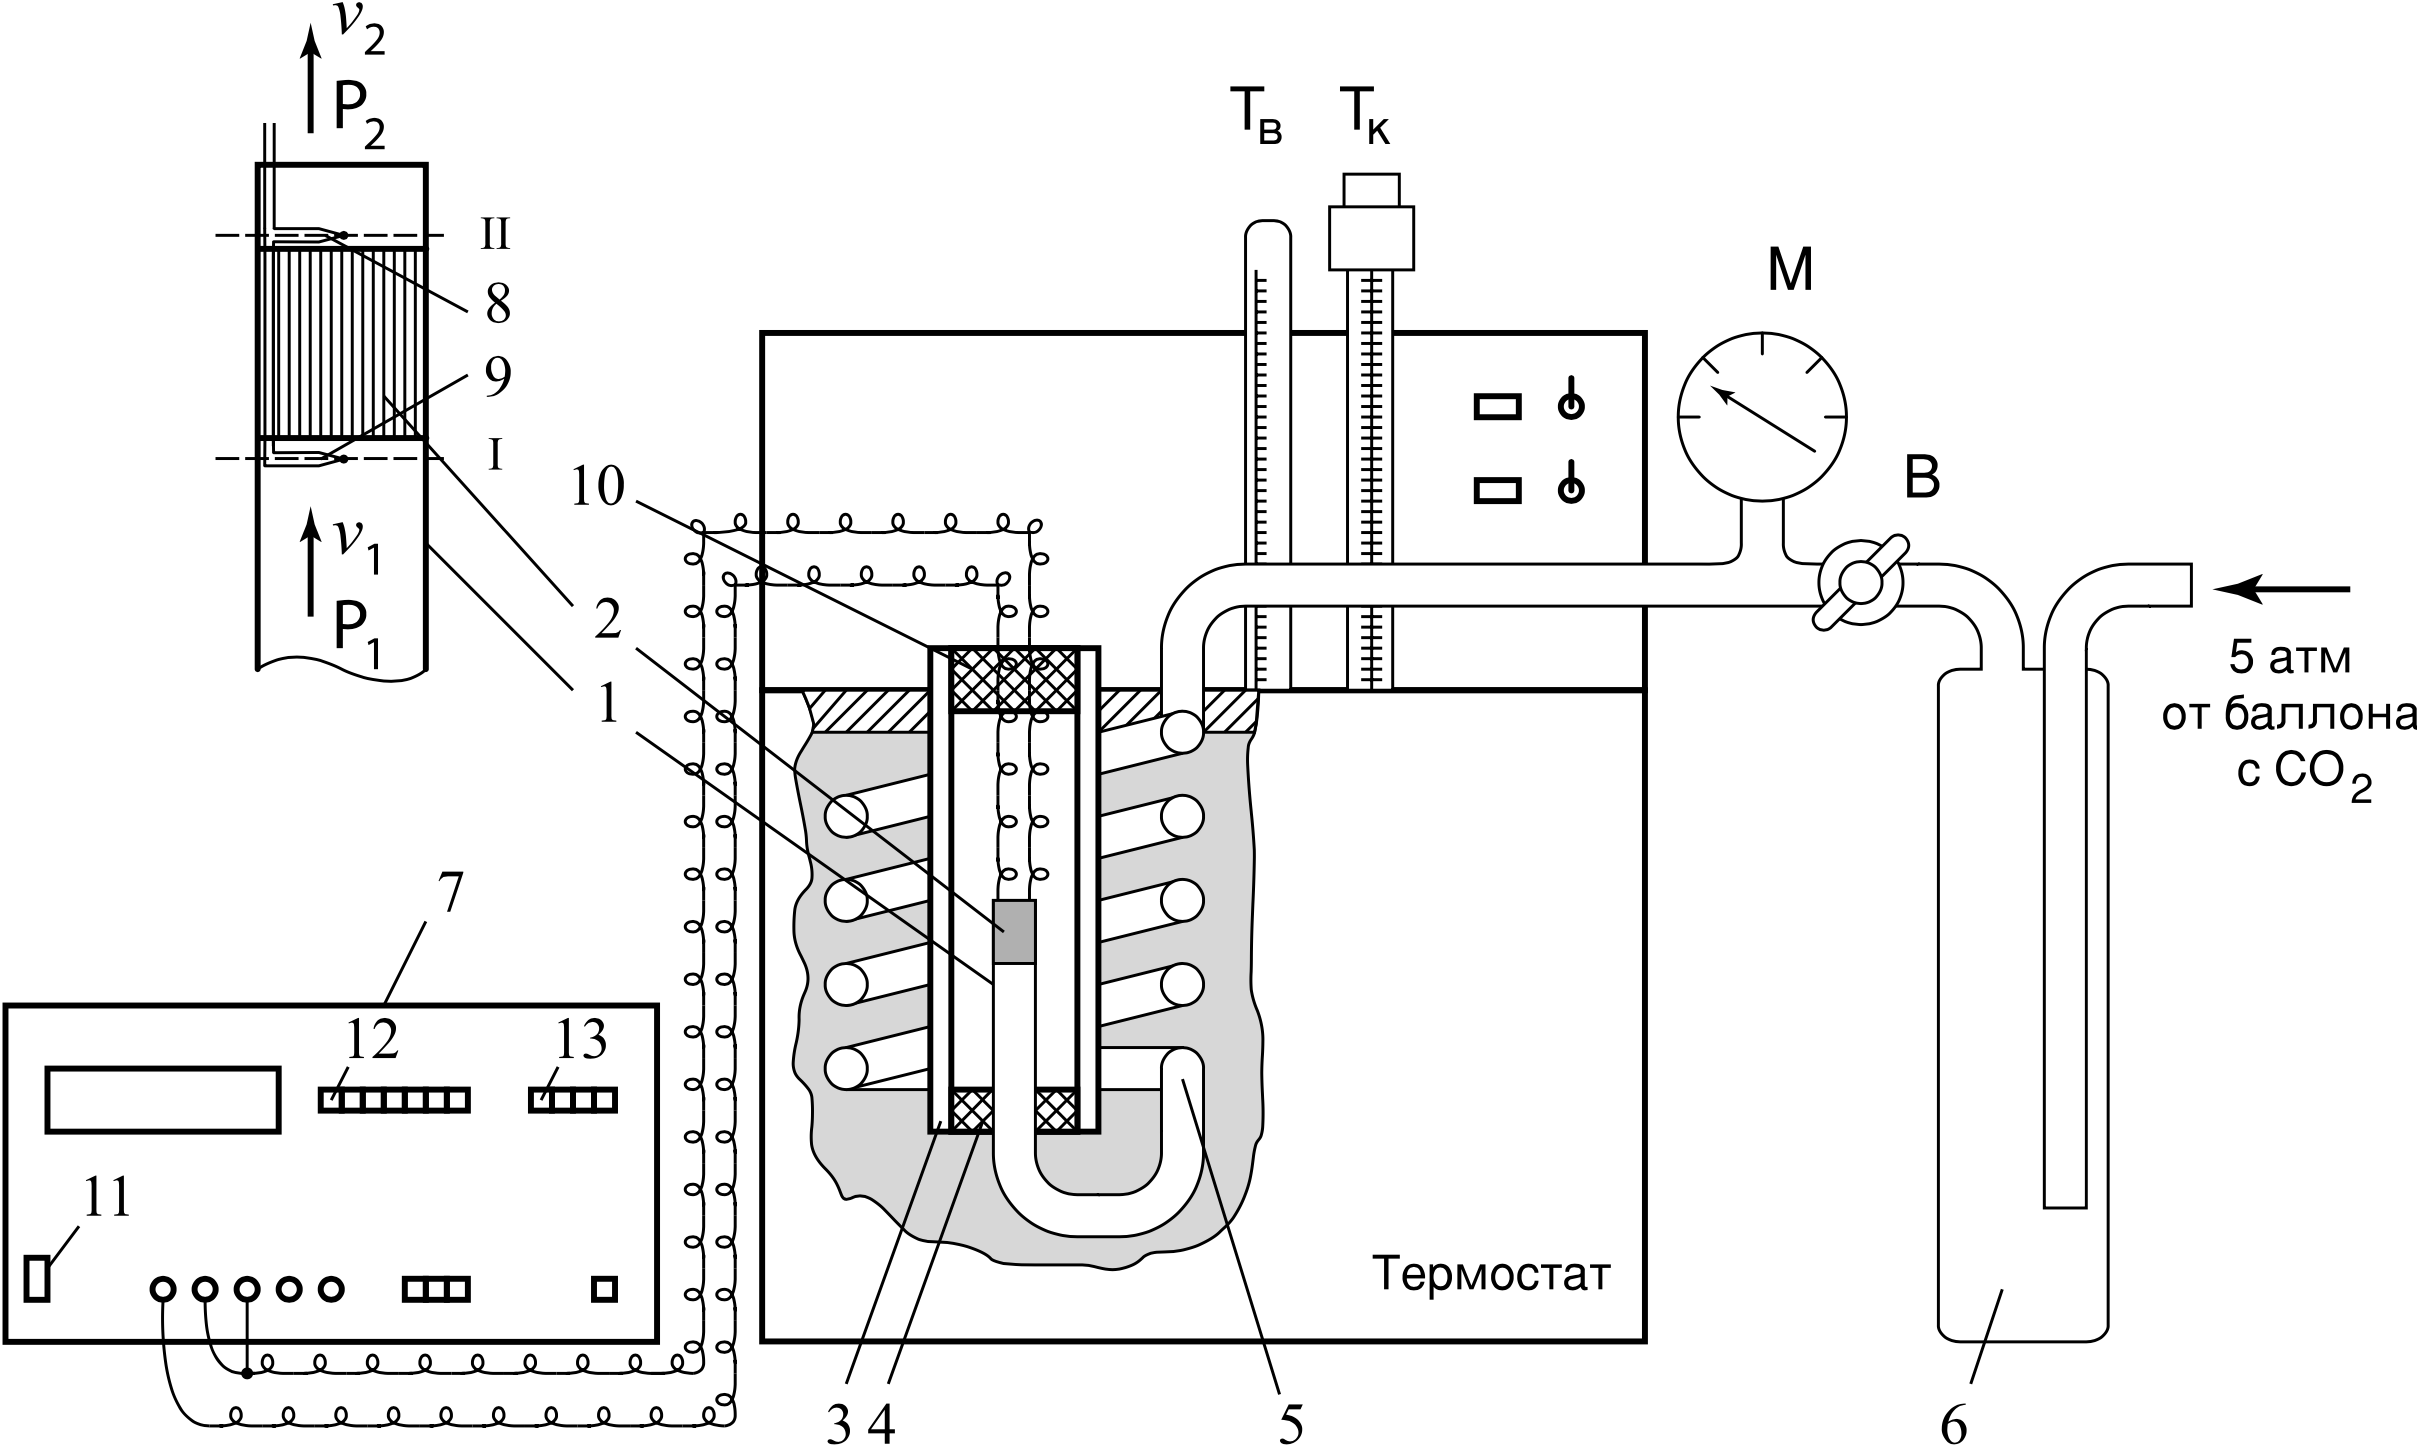
\includegraphics[width=0.9\linewidth]{images/ustanovka.png}
        \caption{Схема установки для изучения эффекта Джоуля-Томсона}
        \label{pic1}
    \end{figure}
    
    Схема установки для исследования эффекта Джоуля–Томсона в углекислом газе представлена на рисунке. Основным элементом установки является трубка 1 с пористой перегородкой 2, через которую пропускается исследуемый газ. Трубка имеет длину $80 \text{ мм}$ и сделана из нержавеющей стали, обладающей, как известно, малой теплопроводностью. Диаметр трубки $d = 3 \text{ мм}$, толщина стенок $0,2 \text{ мм}$. Пористая перегородка расположена в конце трубки и представляет собой стеклянную пористую пробку со множеством узких и длинных каналов. Пористость и толщина пробки ($l = 5 \text{ мм}$) подобраны так, чтобы обеспечить оптимальный поток газа при перепаде давлений $\Delta P \leq 4 \text{ атм}$ (расход газа составляет около $10 \text{ см}^3 \text{/с}$); при этом в результате эффекта Джоуля–Томсона создается достаточная разность температур.
    
    Углекислый газ под повышенным давлением поступает в трубку через змеевик 5 из балластного баллона 6. Медный змеевик омывается водой и нагревает медленно протекающий через него газ до температуры воды в термостате. Температура воды измеряется термометром $T_в$, помещенным в термостате. Требуемая температура воды устанавливается и поддерживается во время эксперимента при помощи контактного термометра $T_к$.
    
    Давление газа в трубке измеряется манометром М и регулируется вентилем В (при открывании вентиля В, т. е. при повороте ручки против часовой стрелки, давление $P_1$ повышается). Манометр М измеряет разность между давлением внутри трубки и наружным (атмосферным) давлением. Так как углекислый газ после пористой перегородки выходит в область с атмосферным давлением $P_2$, то этот манометр непосредственно измеряет перепад давления на входе и на выходе трубки $\Delta P = P_1 - P_2$.
    
    Разность температур газа до перегородки и после нее измеряется дифференциальной термопарой медь — константан. Константановая проволока диаметром $0,1 \text{ мм}$ соединяет спаи 8 и 9, а медные проволоки (того же диаметра) подсоединены к цифровому вольтметру 7. Отвод тепла через проволоку столь малого сечения пренебрежимо мал. Для уменьшения теплоотвода трубка с пористой перегородкой помещена в трубу Дьюара 3, стенки которой посеребрены, для уменьшения теплоотдачи, связанной с излучением. Для уменьшения теплоотдачи за счет конвекции один конец трубы Дьюара уплотнен кольцом 4, а другой закрыт пробкой 10 из пенопласта. Такая пробка практически не создает перепада давлений между внутренней полостью трубы и атмосферой.\\
    
    \begin{flushleft}
        {\Large {\bf Ход работы/Обработка результатов эксперимента}}
    \end{flushleft}
    
    \begin{enumerate}
        
        \item[1.] Запишем погрешности измерительных приборов:
            \begin{itemize}
                \item Вольтметр универсальный B7-78/1: $\varepsilon_U \sim 0,06 \text{ } \%$
                \item Манометр EN-837-1: класс точности – 1, $\sigma_P = \pm 0,02 \text{ } атм.$
                \item Термостат жидкостный ТЖ-ТС-01: $\sigma_T = \pm 0,1^{\circ}\text{C}$
            \end{itemize}
        
        \item[2.] Перед началом работы убедимся в том, что термостат залит водой, а все электрические приборы заземлены. Включим термостат и установим на нём температуру $T = 20^{\circ}\text{C}$.
        
        \item[3.] После установления температуры термостата откроем регулирующий вентиль В настолько, чтобы избыточное давление составило $\Delta P \approx 4 \text{ } атм$.
        
        \item[4.] Через 1,5–2 минуты после подачи давления, когда польностью затухнут переходные процессы, запишем показания вольтметра. Результаты будем заносить в табл. \ref{table1}.
        
        \item[5.] При помощи вентиля В установим давление на 0,5 атм. меньше первоначального. Через 1,5–2 минуты, когда установятся давление и разность температур, вновь запишем показания манометра и вольтметра в табл. \ref{table1}.
        
        \item[6.] Проведём измерения для шести значений давления (от 4 до 1,5 атм) при температуре $T = 20^{\circ}\text{C}$. По ходу выполнения работы не будем забывать переводить показания вольтметра в разность температур по таблице зависимости чувствительности термопары от температуры, приведённой в описании к работе. Результаты занесём в табл. \ref{table1}.
        
        \item[7.] Отложим полученные точки на графике $\Delta T (\Delta P)$, по наклону графика определим коэффициент Джоуля-Томсона для выбранной нами температуры: $\mu_{д-т} = \frac{d(\Delta T)}{d(\Delta P) \cdot 0,968} \text{ } К/атм$.
        
        Погрешность $d(\Delta T)/d(\Delta P)$ рассчитаем по следующим формулам:
        \begin{equation}
            \sigma_{d(\Delta T)/d(\Delta P)}^{случ} = \frac{1}{\sqrt{n}} \sqrt{\frac{\langle (\Delta T)^2 \rangle - \langle \Delta T \rangle^2}{\langle (\Delta P)^2 \rangle - \langle \Delta P \rangle^2} - \left( \frac{d(\Delta T)}{d(\Delta P)} \right)^2}, 
        \end{equation}
        где $n$ — кол-во точек. В нашем случае $n = 6$.
        \begin{equation}
            \varepsilon_{d(\Delta T)/d(\Delta P)}^{приб} = \sqrt{\varepsilon_U^2 + \varepsilon_P^2},
        \end{equation}
        \begin{equation}
            \sigma_{d(\Delta T)/d(\Delta P)} = \sqrt{(\sigma_{d(\Delta T)/d(\Delta P)}^{случ})^2 + (\sigma_{d(\Delta T)/d(\Delta P)}^{приб})^2}.
        \end{equation}
        
        \item[8.] Проделаем измерения пп. 3–7 ещё для 7 значений температур, меняя температуру на $\Delta T = 5^{\circ}\text{C}$ (от $20^{\circ}\text{C}$ до $55^{\circ}\text{C}$).
        
        Все полученные результаты и графики приведём в табл. \ref{table1}.
        
    \end{enumerate}
    
    \begin{table}[pt]

        \begin{minipage}[ht]{0.55\linewidth}
            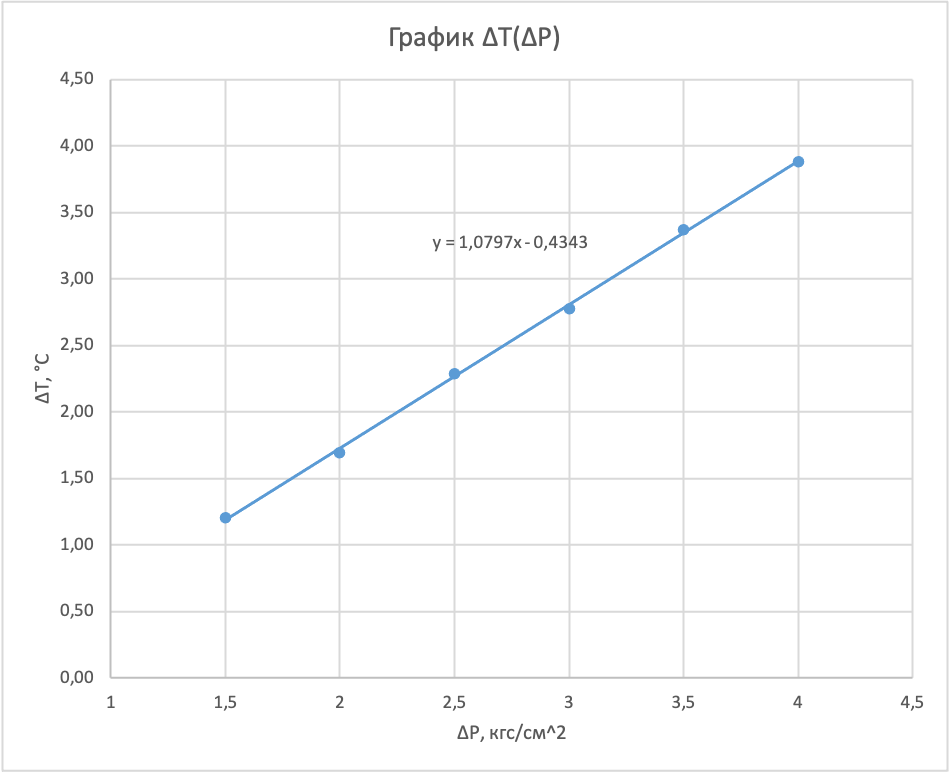
\includegraphics[width=\linewidth]{images/ch1.png}
        \end{minipage}
        \hfill
        \begin{minipage}[ht]{0.47\linewidth}
            \begin{tabular}{|c|c|c|}
                \hline
                \multicolumn{3}{|c|}{$T = 20,2^{\circ}\text{C}$} \\
                \hline
                $\Delta P$, $кгс/см^2$ & $U$, $мкВ$ & $\Delta T$, $^{\circ}\text{C}$ \\
                \hline
                4 & 158 & 3,88 \\
                \hline
                3,5 & 137 & 3,37 \\
                \hline
                3 & 113 & 2,78 \\
                \hline
                2,5 & 93 & 2,29 \\
                \hline
                2 & 69 & 1,70 \\
                \hline
                1,5 & 49 & 1,20 \\
                \hline
                $\mu_{д-т}$, К/атм & $\sigma_{\mu_{д-м}}$, К/атм & $\varepsilon_{\mu_{д-т}}$, \% \\
                \hline
                1,12 & 0,01 & 1,2 \\
                \hline
            \end{tabular}
        \end{minipage}
        
        \vspace{0.5cm}
        
        \begin{minipage}[ht]{0.55\linewidth}
            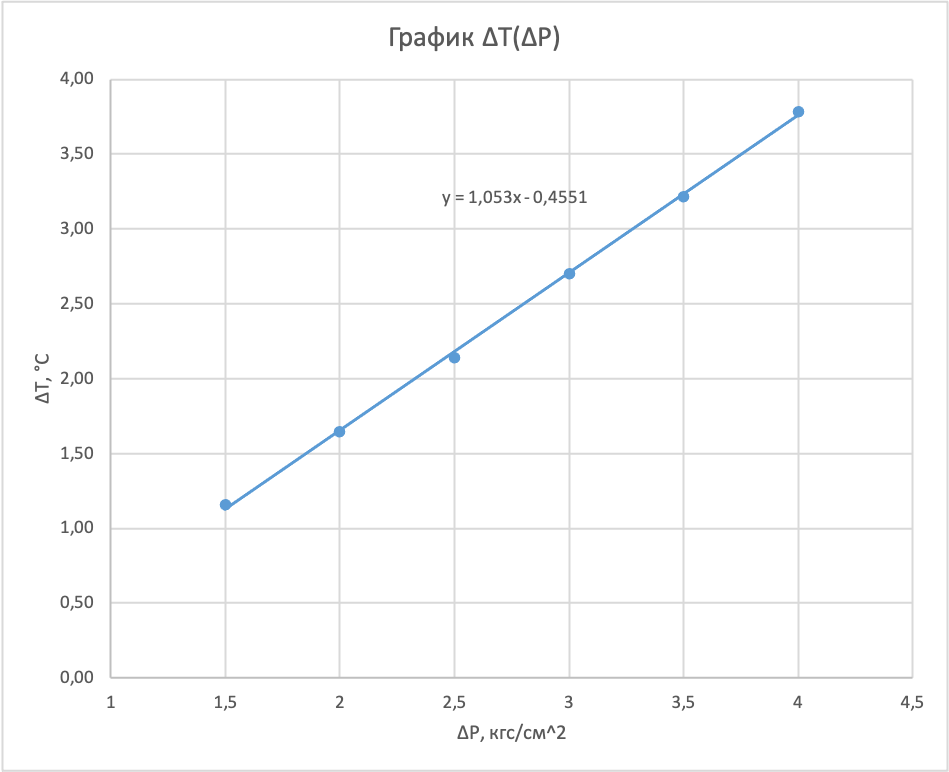
\includegraphics[width=\linewidth]{images/ch2.png}
        \end{minipage}
        \hfill
        \begin{minipage}[ht]{0.47\linewidth}
            \begin{tabular}{|c|c|c|}
                \hline
                \multicolumn{3}{|c|}{$T = 25,0^{\circ}\text{C}$} \\
                \hline
                $\Delta P$, $кгс/см^2$ & $U$, $мкВ$ & $\Delta T$, $^{\circ}\text{C}$ \\
                \hline
                4 & 154 & 3,78 \\
                \hline
                3,5 & 131 & 3,22 \\
                \hline
                3 & 110 & 2,70 \\
                \hline
                2,5 & 87 & 2,14 \\
                \hline
                2 & 67 & 1,65 \\
                \hline
                1,5 & 47 & 1,15 \\
                \hline
                $\mu_{д-т}$, К/атм & $\sigma_{\mu_{д-м}}$, К/атм & $\varepsilon_{\mu_{д-т}}$, \% \\
                \hline
                1,09 & 0,01 & 1,3 \\
                \hline
            \end{tabular}
        \end{minipage}
        
        \vspace{0.5cm}
        
        \begin{minipage}[ht]{0.55\linewidth}
            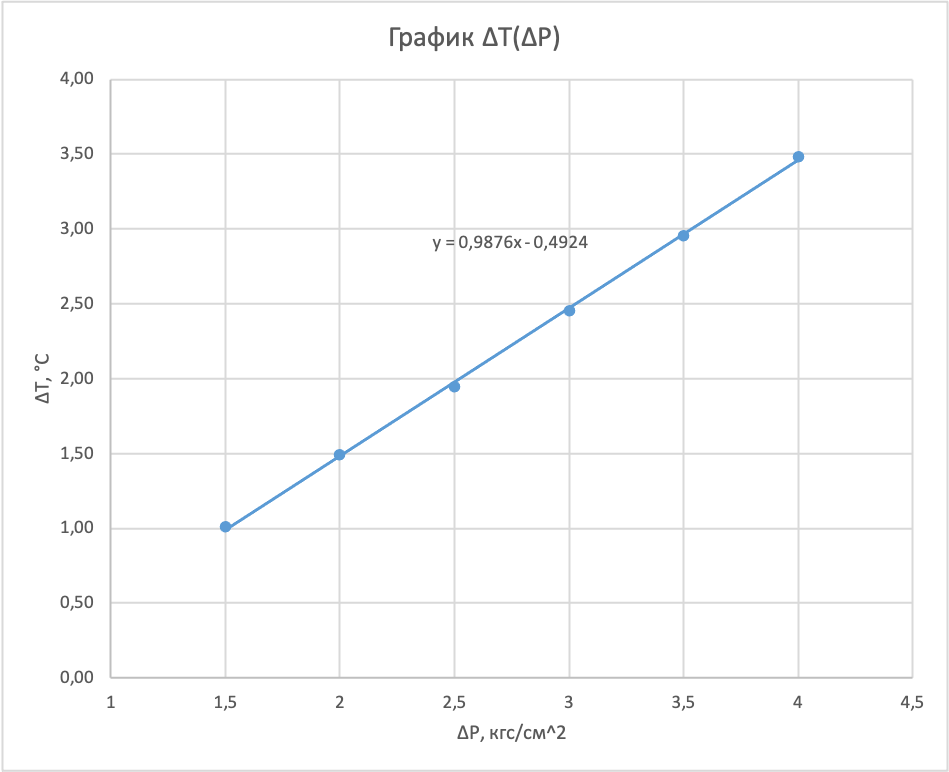
\includegraphics[width=\linewidth]{images/ch3.png}
        \end{minipage}
        \hfill
        \begin{minipage}[ht]{0.47\linewidth}
            \begin{tabular}{|c|c|c|}
                \hline
                \multicolumn{3}{|c|}{$T = 30,0^{\circ}\text{C}$} \\
                \hline
                $\Delta P$, $кгс/см^2$ & $U$, $мкВ$ & $\Delta T$, $^{\circ}\text{C}$ \\
                \hline
                4 & 145 & 3,49 \\
                \hline
                3,5 & 123 & 2,96 \\
                \hline
                3 & 102 & 2,45 \\
                \hline
                2,5 & 81 & 1,95 \\
                \hline
                2 & 62 & 1,49 \\
                \hline
                1,5 & 42 & 1,01 \\
                \hline
                $\mu_{д-т}$, К/атм & $\sigma_{\mu_{д-м}}$, К/атм & $\varepsilon_{\mu_{д-т}}$, \% \\
                \hline
                1,02 & 0,01 & 1,2 \\
                \hline
            \end{tabular}
        \end{minipage}
        
    \end{table}
    
    \begin{table}[pt]
        
        \begin{minipage}[ht]{0.55\linewidth}
            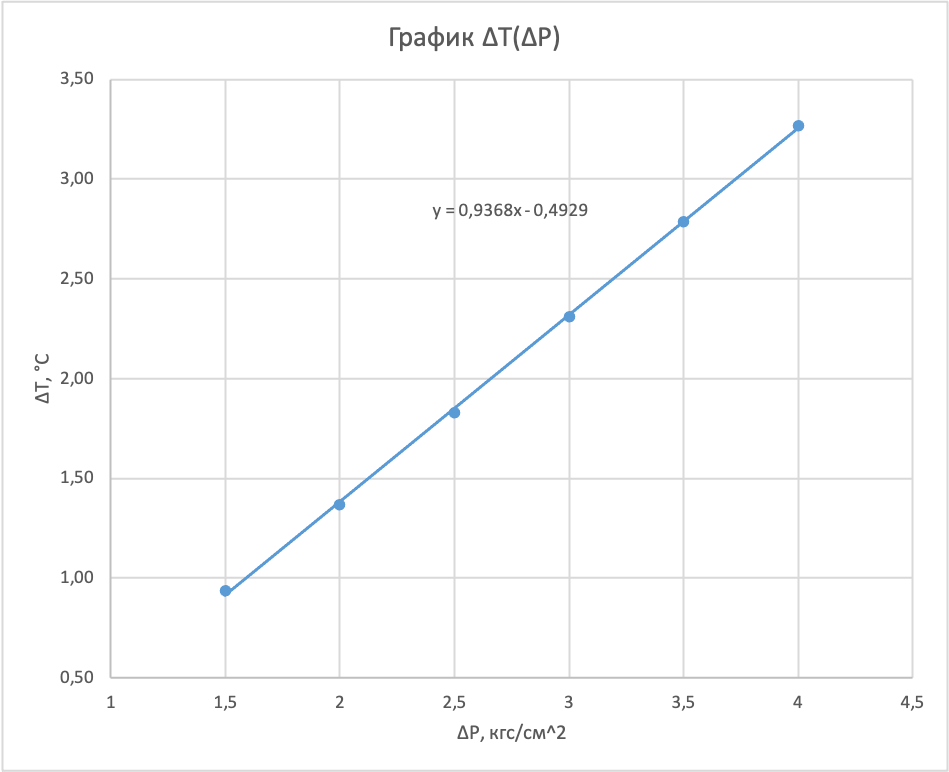
\includegraphics[width=\linewidth]{images/ch4.png}
        \end{minipage}
        \hfill
        \begin{minipage}[ht]{0.47\linewidth}
            \begin{tabular}{|c|c|c|}
                \hline
                \multicolumn{3}{|c|}{$T = 35,0^{\circ}\text{C}$} \\
                \hline
                $\Delta P$, $кгс/см^2$ & $U$, $мкВ$ & $\Delta T$, $^{\circ}\text{C}$ \\
                \hline
                4 & 136 & 3,27 \\
                \hline
                3,5 & 116 & 2,79 \\
                \hline
                3 & 96 & 2,31 \\
                \hline
                2,5 & 76 & 1,83 \\
                \hline
                2 & 57 & 1,37 \\
                \hline
                1,5 & 39 & 0,94 \\
                \hline
                $\mu_{д-т}$, К/атм & $\sigma_{\mu_{д-м}}$, К/атм & $\varepsilon_{\mu_{д-т}}$, \% \\
                \hline
                0,97 & 0,01 & 1,1 \\
                \hline
            \end{tabular}
        \end{minipage}
        
        \vspace{0.5cm}
        
        \begin{minipage}[ht]{0.55\linewidth}
            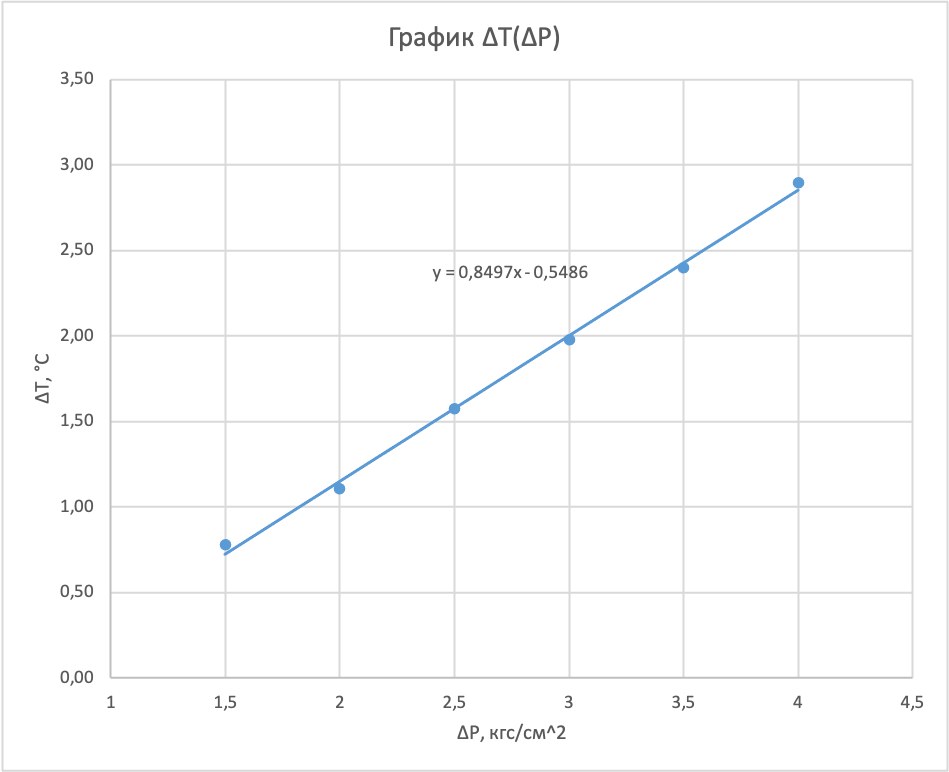
\includegraphics[width=\linewidth]{images/ch5.png}
        \end{minipage}
        \hfill
        \begin{minipage}[ht]{0.47\linewidth}
            \begin{tabular}{|c|c|c|}
                \hline
                \multicolumn{3}{|c|}{$T = 40,1^{\circ}\text{C}$} \\
                \hline
                $\Delta P$, $кгс/см^2$ & $U$, $мкВ$ & $\Delta T$, $^{\circ}\text{C}$ \\
                \hline
                4 & 123 & 2,89 \\
                \hline
                3,5 & 102 & 2,40 \\
                \hline
                3 & 84 & 1,98 \\
                \hline
                2,5 & 67 & 1,58 \\
                \hline
                2 & 47 & 1,11 \\
                \hline
                1,5 & 33 & 0,78 \\
                \hline
                $\mu_{д-т}$, К/атм & $\sigma_{\mu_{д-м}}$, К/атм & $\varepsilon_{\mu_{д-т}}$, \% \\
                \hline
                0,88 & 0,02 & 2,1 \\
                \hline
            \end{tabular}
        \end{minipage}
        
        \vspace{0.5cm}
        
        \begin{minipage}[ht]{0.55\linewidth}
            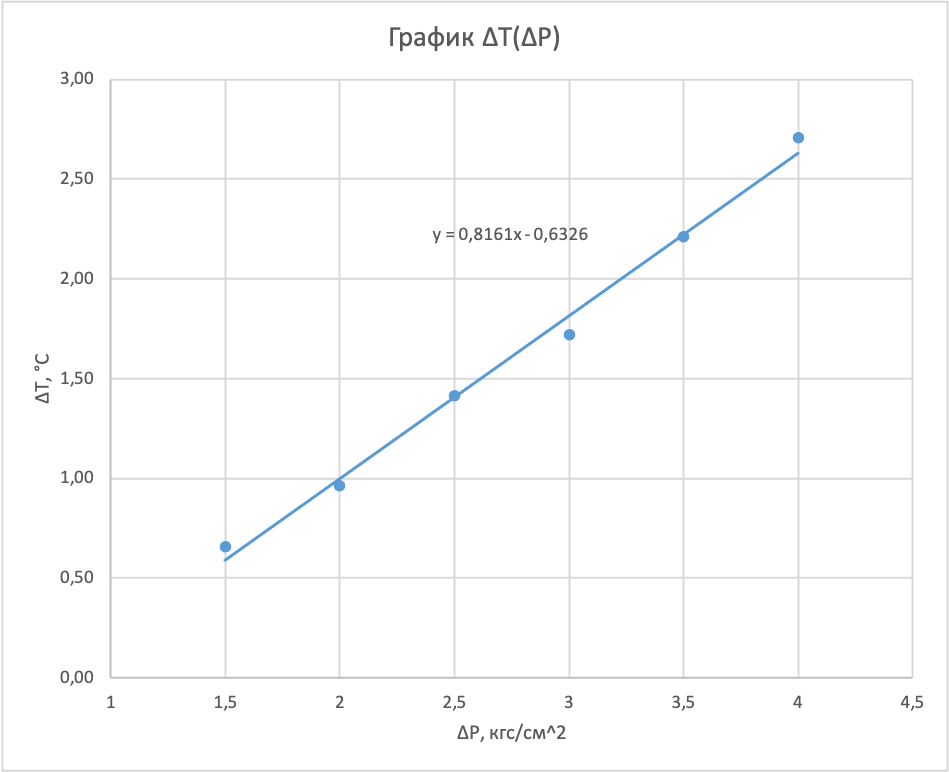
\includegraphics[width=\linewidth]{images/ch6.png}
        \end{minipage}
        \hfill
        \begin{minipage}[ht]{0.47\linewidth}
            \begin{tabular}{|c|c|c|}
                \hline
                \multicolumn{3}{|c|}{$T = 45,2^{\circ}\text{C}$} \\
                \hline
                $\Delta P$, $кгс/см^2$ & $U$, $мкВ$ & $\Delta T$, $^{\circ}\text{C}$ \\
                \hline
                4 & 115 & 2,71 \\
                \hline
                3,5 & 94 & 2,21 \\
                \hline
                3 & 73 & 1,72 \\
                \hline
                2,5 & 60 & 1,41 \\
                \hline
                2 & 41 & 0,96 \\
                \hline
                1,5 & 28 & 0,66 \\
                \hline
                $\mu_{д-т}$, К/атм & $\sigma_{\mu_{д-м}}$, К/атм & $\varepsilon_{\mu_{д-т}}$, \% \\
                \hline
                0,84 & 0,03 & 3,5 \\
                \hline
            \end{tabular}
        \end{minipage}
        
    \end{table}
    
    \begin{table}[pt]
        \captionsetup{justification=centering, margin=2cm}
        
        \begin{minipage}[ht]{0.55\linewidth}
            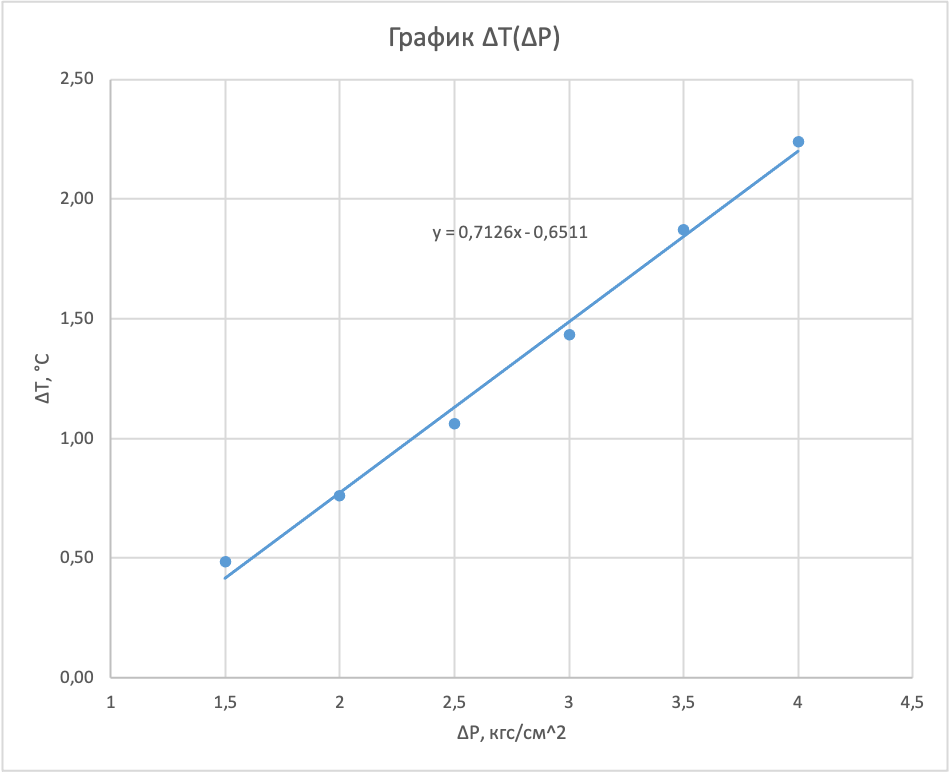
\includegraphics[width=\linewidth]{images/ch7.png}
        \end{minipage}
        \hfill
        \begin{minipage}[ht]{0.47\linewidth}
            \begin{tabular}{|c|c|c|}
                \hline
                \multicolumn{3}{|c|}{$T = 50,1^{\circ}\text{C}$} \\
                \hline
                $\Delta P$, $кгс/см^2$ & $U$, $мкВ$ & $\Delta T$, $^{\circ}\text{C}$ \\
                \hline
                4 & 97 & 2,24 \\
                \hline
                3,5 & 81 & 1,87 \\
                \hline
                3 & 62 & 1,43 \\
                \hline
                2,5 & 46 & 1,06 \\
                \hline
                2 & 33 & 0,76 \\
                \hline
                1,5 & 21 & 0,48 \\
                \hline
                $\mu_{д-т}$, К/атм & $\sigma_{\mu_{д-м}}$, К/атм & $\varepsilon_{\mu_{д-т}}$, \% \\
                \hline
                0,74 & 0,03 & 3,4 \\
                \hline
            \end{tabular}
        \end{minipage}
        
        \vspace{0.5cm}
        
        \begin{minipage}[ht]{0.55\linewidth}
            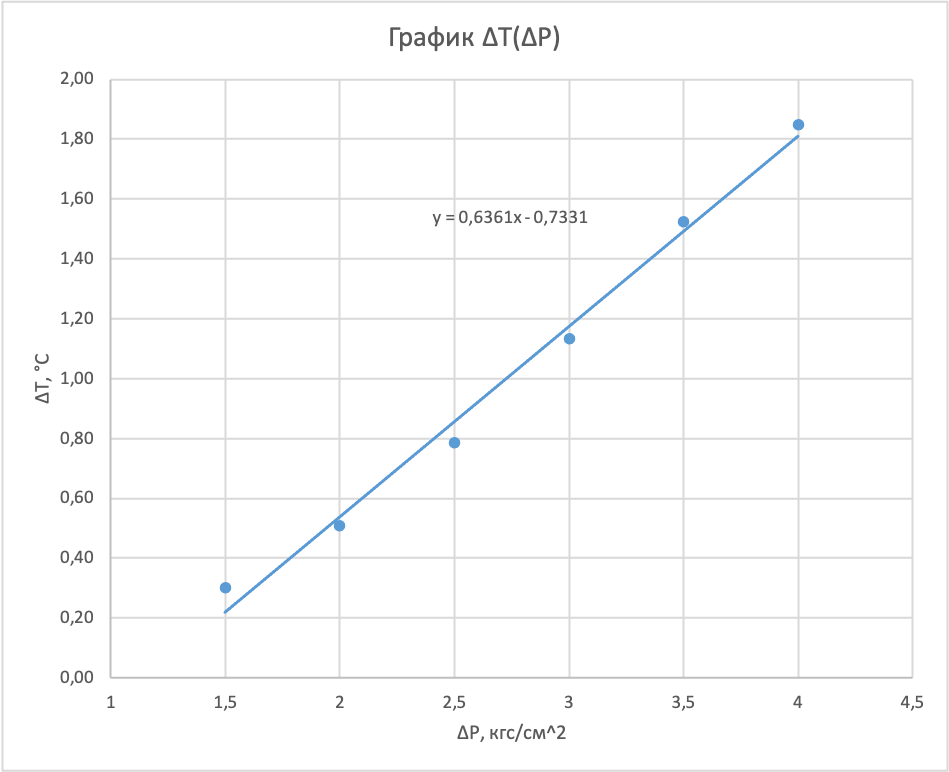
\includegraphics[width=\linewidth]{images/ch8.png}
        \end{minipage}
        \hfill
        \begin{minipage}[ht]{0.47\linewidth}
            \begin{tabular}{|c|c|c|}
                \hline
                \multicolumn{3}{|c|}{$T = 55,0^{\circ}\text{C}$} \\
                \hline
                $\Delta P$, $кгс/см^2$ & $U$, $мкВ$ & $\Delta T$, $^{\circ}\text{C}$ \\
                \hline
                4 & 80 & 1,85 \\
                \hline
                3,5 & 66 & 1,52 \\
                \hline
                3 & 49 & 1,13 \\
                \hline
                2,5 & 34 & 0,79 \\
                \hline
                2 & 22 & 0,51 \\
                \hline
                1,5 & 13 & 0,30 \\
                \hline
                $\mu_{д-т}$, К/атм & $\sigma_{\mu_{д-м}}$, К/атм & $\varepsilon_{\mu_{д-т}}$, \% \\
                \hline
                0,66 & 0,03 & 4,0 \\
                \hline
            \end{tabular}
        \end{minipage}
        
        \caption{Графики зависимости $\Delta T$ от $\Delta P$ и значения коэффициента Джоуля-Томсона при разных температурах}
        \label{table1}
        
    \end{table}
    
    \newpage
    
    \begin{enumerate}
    
        \item[9.] Пользуясь данными табл. \ref{table1}, построим график зависимости $\mu_{д-т}(1/T)$. Результат представим в табл. \ref{table2}.
        
        \begin{figure}[ht]
            \centering
            \includegraphics[width=0.85\linewidth]{images/µ(1:T).png}
        \end{figure}
        
        \begin{table}[ht]
            \centering
            \begin{tabular}{|c|c|c|c|c|c|c|c|c|}
                \hline
                $\mu_{д-т}$, К/атм & 1,12 & 1,09 & 1,02 & 0,97 & 0,88 & 0,84 & 0,74 & 0,66 \\
                \hline
                $1/T \cdot 10^3$, $К^{-1}$ & 3,41 & 3,36 & 3,30 & 3,25 & 3,19 & 3,14 & 3,10 & 3,05 \\
                \hline
            \end{tabular}
            \caption{График зависимости $\mu_{д-т}$ от $1/T$}
            \label{table2}
        \end{table}
        
        \item[10.] Пользуясь графиком, приведённом в табл. \ref{table2}, найдём значения постоянных $a$ и $b$ для углекислого газа:
        
        По формуле \eqref{eq3} видно, что:
        \begin{equation}
            \frac{d(\mu_{д-т})}{d(1/T)} = \frac{2a}{R C_p},
        \end{equation}
        откуда
        \begin{equation}
            a = \frac{d(\mu_{д-т})}{d(1/T)} \cdot \frac{R C_p}{2}.
        \end{equation}
        Погрешность $a$ рассчитаем по следующим формулам:
        \begin{equation}
            \sigma_{d(\mu_{д-т})/d(1/T)}^{случ} = \frac{1}{\sqrt{n}} \sqrt{\frac{\langle \mu_{д-т}^2 \rangle - \langle \mu_{д-т} \rangle^2}{\langle (1/T)^2 \rangle - \langle 1/T \rangle^2} - \left( \frac{d(\mu_{д-т})}{d(1/T)} \right)^2},
        \end{equation}
        \begin{equation}
            \varepsilon_a^{случ} = \varepsilon_{d(\mu_{д-т})/d(1/T)}^{случ},
        \end{equation}
        \begin{equation}
            \varepsilon_a^{приб} = \sqrt{(\varepsilon_{d(\Delta T)/d(\Delta P)}^{приб})^2 + (\varepsilon_T)^2},
        \end{equation}
        \begin{equation}
            \sigma_a = \sqrt{(\sigma_a^{случ})^2 + (\sigma_a^{приб})^2}.
        \end{equation}
        В итоге получим
        \begin{equation}
            a = (1,95 \pm 0,09) \text{ } \frac{\text{Н} \cdot \text{м}^4}{\text{моль}^2}
        \end{equation}
        
        \newpage
        
        Экстраполируя график зависимости $\mu_{д-т}(1/T)$, найдём значение $\mu_0$ — значение $\mu_{д-т}$ при пересечении оси ординат. По формуле \eqref{eq3} видно, что:
        \begin{equation}
            \mu_0 = -\frac{b}{C_p},
        \end{equation}
        тогда
        \begin{equation}
            b = -\mu_0 \cdot C_p.
        \end{equation}
        Погрешности рассчитаем по следующим формулам:
        \begin{equation}
            \varepsilon_{\mu_0}^{приб} = \varepsilon_{d(\Delta T)/d(\Delta P)}^{приб},
        \end{equation}
        \begin{equation}
            \sigma_{\mu_0} = \sqrt{(\sigma_{\mu_0}^{случ})^2 + (\sigma_{\mu_0}^{приб})^2},
        \end{equation}
        \begin{equation}
            \varepsilon_b = \varepsilon_{\mu_0}.
        \end{equation}
        Случайную погрешность $\mu_0$ посчитаем по МНК. В итоге получим
        \begin{equation}
            b = (11,9 \pm 0,3) \cdot 10^{-4} \text{ } \frac{\text{м}^3}{\text{моль}}
        \end{equation}
        
        \item[11.] Найдём $T_{инв}$ для углекислого газа:
        \begin{equation}
            T_{инв} = \frac{2a}{R b},
        \end{equation}
        \begin{equation}
            \varepsilon_{T_{инв}} = \sqrt{\varepsilon_a^2 + \varepsilon_b^2}.
        \end{equation}
        В итоге получим
        \begin{equation}
            T_{инв} = (3,9 \pm 0,2) \cdot 10^2 \text{ К}.
        \end{equation}\\
    
    \end{enumerate}
    
    \begin{flushleft}
        {\Large {\bf Вывод}}
    \end{flushleft}
    
    В данной работе была получена зависимость коэффициента Джоуля-Томсона от температуры для углекислого газа. Также были найдены значения постоянных в уравнении Ван-дер-Ваальса для углекислого газа и получена температура инверсии для углекислого газа. Как и следовало ожидать, значения не совпали с табличными в пределах погрешности, что говорит о том, что модель Ван-дер-Ваальса плохо количественно описывает действительность, однако качественно она же всё хорошо предугадывает.
    
\end{document}